%%%%%%%%%%%%%%%%%%%%%%%%%%%%%%%%%%%%%%%
\chapter{Dynamics of charged particles with arbitrary magnetic moment}
\label{chap:moment}
%%%%%%%%%%%%%%%%%%%%%%%%%%%%%%%%%%%%%%%
\noindent In \rsec{sec:mom}, we addressed two different models of introducing anomalous magnetic moment in QM: 
\begin{enumerate}
\item[(a)] the Dirac-Pauli (DP) first order equation which is the Dirac equation where $g$-factor is precisely fixed to the $g\!=\!2$, with the addition of an incremental Pauli term; and
\item[(b)] the Klein-Gordon-Pauli (KGP) second order equation which \lq\lq squares\rq\rq\ the Dirac equation and thereafter allows the magnetic moment $\bb{\mu}$ to vary independently of charge and mass, unlike Dirac theory.
\end{enumerate} 
These two approaches coincide when the anomaly $a$ vanishes. However, all particles that have magnetic moments differ from the Dirac value $g\!=\!2$, either due to their composite nature, or, for point particles, due to the quantum vacuum fluctuation effect.

We find that even a small magnetic anomaly has a large effect in the limit of strong fields generated by massive magnetar stars~\citep{Kaspi:2017fwg}. Therefore it is not clear that the tacit assumption of $g\!=\!2$ in the case of strong fields~\citep{Rafelski:1976ts,Greiner:1985ce,Rafelski:2016ixr} is prudent~\citep{Evans:2018kor}. This argument is especially applicable to tightly bound composite particles such as protons and neutrons where the large anomalous magnetic moment can be taken as an external prescribed parameter unrelated to the elementary quantum vacuum fluctuations. It is then of particular interest to study the dynamical behavior of these particles in fields of magnetar strength. This interest carries over to the environment of strong fields created in focus of ultra-intense laser pulses and the associated particle production processes~\citep{Dunne:2014qda,Hegelich:2014tda}. We consider also precision spectroscopic experiments and recognize consequences even in the weak coupling limit.

This chapter reviews our work done in exploring relativistic dynamics with arbitrary magnetic dipoles in both a quantum mechanical and classical context. \rsec{sec:homogeneous} and \rsec{sec:coulomb} is primarily based on~\cite{Steinmetz:2018ryf} and covers analytic solutions for the Klein-Gordon-Pauli (KGP) equation in the presence of homogeneous magnetic fields and the Coulomb problem for hydrogen-like atoms. Comparisons with the Dirac-Pauli (DP) and Dirac solutions are made and novel consequences for strong fields are discussed in \rsec{sec:sb}.

\rsec{sec:kgptopics} covers special topics related to KGP including a proposal which couples mass and magnetic moment (\rsec{sec:ikgp}) and an extension to particles (such as quarks) which are charged under both Albelian and non-Albelian fields (\rsec{sec:quarks}). The second special topic is yet unpublished outside this dissertation.

Relativistic classical spin dynamics is discussed in \rsec{sec:cspin} and is based on our work in~\cite{Rafelski:2017hce}. We propose in \rsec{sec:magpotential} a covariant form of magnetic dipole potential which modifies the Lorentz force, extends the Thomas-Bargmann-Michel-Telegdi (TMBT) equation, and reproduces the Stern-Gerlach force in the non-relativistic limit. %\rsec{sec:ampgil} discusses our finding that this magnetic potential also serves to unify both the Amp{\`e}rian and Gilbertian pictures of dipole moments.

%%%%%%%%%%%%%%%%%%%%%%%%%%%%%%%%%%%%%%%
\section{Homogeneous magnetic fields}
\label{sec:homogeneous}
%%%%%%%%%%%%%%%%%%%%%%%%%%%%%%%%%%%%%%%
\noindent The case of the homogeneous magnetic field, sometimes referred to as the Landau problem, provides a stepping stone in which to examine the consequences of quantum spin dynamics in a concrete analytical fashion. We present here an abbreviated analysis and the full treatment of this solution in terms of Ladder operators can be found in~\cite{Steinmetz:2018ryf} while alternative approaches are shown in texts such as~\cite{Itzykson:1980rh}. We take a constant magnetic field in the $z$-direction to be
\begin{alignat}{1}
	\label{homogeneous:1} \bb{B}=(0,0,B)\,.
\end{alignat}
For our choice of gauge, there are two common options: (a) the Landau $\bb{A}_\mathrm{L}$ gauge and (b) the symmetric $\bb{A}_\mathrm{S}$ gauge
\begin{alignat}{1}
	\label{homogeneous:2} \bb{A}_\mathrm{L}=B(0,x,0)\,,\indent \bb{A}_\mathrm{S}=\frac{B}{2}(-y,x,0)\,.
\end{alignat}
As the system has a manifest rotational symmetry perpendicular to the direction of the homogeneous field, we will choose the symmetric gauge $\bb{A}_\mathrm{S}$ which preserves this symmetry explicitly.

Before we examine relativistic wave equations, it will be helpful to first consider the non-relativistic Schr{\"o}dinger-Pauli case as the KGP-Landau problem can be written as equivalent to the Schro{\"o}dinger-Pauli Hamiltonian. We consider energy eigenstates of and electron with $m_{e}$ described by \req{sp:1} under \req{homogeneous:1} as
\begin{alignat}{1}
	\label{homogeneous:3} \chi\rightarrow\chi_\mathrm{E}\exp\left(-\frac{iEt}{\hbar}\right)\,,\qquad\left(\frac{1}{2m_{e}}\bb{\pi}^{2}-\bb{\mu}\cdot\bb{B}\right)\chi_\mathrm{E}=E\chi_\mathrm{E}\,,
\end{alignat}
where $\mu$ is the magnitude of the magnetic moment as defined in \req{mag:3}. \req{homogeneous:3} can be further rewritten using angular momentum $\bb{L}$ and the symmetric gauge \req{homogeneous:2} as
\begin{gather}
	\label{homogeneous:4} \left(\frac{1}{2m_{e}}\bb{p}^{2}+\frac{e^{2}B^{2}}{8m_{e}}(x^{2}+y^{2})-\frac{eB}{2m_{e}}L_{3}-\mu B\sigma_{3}\right)\chi_\mathrm{E}=E\chi_\mathrm{E}\,,\\
    \bb{L}=\bb{r}\times\bb{p}\,,\qquad L_{i}=\varepsilon_{ijk}x_{j}p_{k}\,.
\end{gather}

The above can be broken into a set of three mutually commuting Hamiltonian operators: (a) the free particle Hamiltonian, (b) the quantum harmonic oscillator (HO), and (c) the Zeeman interaction (ZI) given by
\begin{align}
	\label{homogeneous:7}
    &H_\mathrm{total}=H_\mathrm{Free}+H_\mathrm{HO}+H_\mathrm{Mag.}\,,\\
	\label{homogeneous:7a}
    &H_{\mathrm{Free}}=\frac{p_{3}^{2}}{2m}\,,\\
	\label{homogeneous:7b}
    &H_\mathrm{HO}\,=\frac{1}{2m_{e}}\left(p_{1}^{2}+p_{2}^{2}\right) + \frac{1}{2}m_{e}\omega^{2}(x^{2}+y^{2})\,,\\
	\label{homogeneous:7c}
    &H_{\mathrm{ZI}}\ \,=-\mu_{B}B\frac{L_{3}}{\hbar}-\mu B\sigma_{3}\,.
\end{align}
The cyclotron frequency appears in \req{homogeneous:7b} as $2\omega=\omega_\mathrm{C}=eB/m_{e}$. We note that the Zeeman \req{homogeneous:7c} is usually expressed as
\begin{alignat}{1}
	\label{homogeneous:7d}
    H_{\mathrm{ZI}}=-\frac{e}{2m}\left(g_\mathrm{L}\bb{L}+g\bb{S}\right)\cdot\bb{B}\,,\qquad g_\mathrm{L}=1\,,
\end{alignat}
with $\bb{S}$ defined in \req{qspin:1}. We see more explicitly that the orbital gyromagnetic ratio $g_\mathrm{L}$ which is a coefficient to the angular momentum operator $\bb{L}$ is unity unlike for spin. We refer back to our comment about black hole spin in \rsec{sec:unique}. As all the above Hamiltonian operators are mutually commuting, the energy eigenvalue of the total Hamiltonian is the sum of the individual energy eigenvalues. Our remaining goal will be to convert the KGP eigenvalue equation into the above three non-relativistic Hamiltonian operators. 

We now return to the KGP equation and write expand \req{kgp:1} for the Landau problem with energy eigenstates $\Psi_\mathrm{E}$ yielding
\begin{alignat}{1}
    \label{lan09}
    \left(\frac{E^{2}}{c^{2}}-m_{e}^{2}c^{2}-\bb{p}^{2}-\frac{1}{4}e^{2}B^{2}\left(x^{2}+y^{2}\right)+eBL_{3}+2\mu m_{e} B\sigma_{3}\right)\Psi_\mathrm{E}=0\;.
\end{alignat} 
We introduce the substitutions 
\begin{alignat}{1}
    \label{lan10}
    E\to m^\prime c^{2}\,,\quad \frac{E^{2}-m_{e}^{2}c^{4}}{2E}\to E^\prime\;,
\end{alignat} 
and recast KGP \req{lan09} into a Schr{\"o}dinger-style Hamiltonian equation
\begin{gather}
	\label{lan11} \left(\frac{1}{2m'}\bb{p}^{2}+\frac{e^{2}B^{2}}{8m'}(x^{2}+y^{2})-\frac{eB}{2m'}L_{3}-\mu\left(\frac{m_{e}}{m'}\right)B\sigma_{3}\right)\Psi_\mathrm{E}=E'\Psi_\mathrm{E}\,,
\end{gather}
which matches the non-relativistic Hamiltonian presented in \req{homogeneous:7}.

The energy eigenvalues of \req{homogeneous:7} are given by
\begin{alignat}{1}
    \label{lan23}
    E^\prime_{n,s}(p_{3},B)&=\frac{p_{3}^{2}}{2m^\prime }+\frac{e\hbar B}{m^\prime}\left(n+\frac{1}{2}\right)-\mu B\left(\frac{m_{e}}{m'}\right)s\,,
\end{alignat}
where $n\in1,2,3\ldots$ is the Landau orbital quantum number and $s\in\pm1$ is the spin quantum number. The physical relativistic energies can be obtained by undoing the substitutions in \req{lan10} yielding from \req{lan23}
\begin{gather}
\label{lan24}
E^{2}_{n,s}(p_{3},B)=m_{e}^{2}c^{4}+p_{3}^{2}c^{2}+2e\hbar c^{2}B\left(n+\frac{1}{2}\right)-2\mu B m_{e}c^{2}s\,,\\
\label{lan24b}
E_{n,s}=\pm\sqrt{m_{e}^{2}c^{4}+p_{3}^{2}c^{2}+2e\hbar c^{2}B\left(n+\frac{1}{2}\right)-2\mu B m_{e}c^{2}s}\;.
\end{gather}
This expression for the relativistic Landau levels is the same as found by ~\cite{Weisskopf:1936hya} for the Dirac equation setting $g\!=\!2$ in \req{lan24b}. The Landau orbital part and spin portions can be combined when the magnetic moment is expressed in terms of $e/m$, but the form in \req{lan24b} keeps it generalized for the case of neutral particles.

The `Landau' problem for neutral particles (for example the neutron with mass $m_\mathrm{N}$) simplifies to
\begin{gather}
\label{neutral:1}
E_{n,s}|_{e=0}\rightarrow E_{s}(\bb{p},B)=\sqrt{m_\mathrm{N}^{2}c^{4}+\bb{p}^{2}c^{2}-2\mu B m_\mathrm{N}c^{2}s}\;,
\end{gather}
which is just the free particle motion with a magnetic dipole energy. We note the correspondence between the quantized Landau orbitals and continuous transverse momentum $\bb{p}^{2}=p_{3}^{2}+p_\mathrm{T}^{2}$. We can define an `effective' polarization mass given by
\begin{gather}
\label{neutral:2}
\boxed{\tilde{m}^{2}_{s}(B)=m^{2}c^{4}-2\mu B mc^{2}s}\,.
\end{gather}
This effective polarization mass (which also is easily defined for charged particles) will find use when we consider cosmic thermodynamics and plasmas in \rchap{chap:cosmo}.

Restricting ourselves to the positive energy spectrum, the non-relativistic reduction of \req{lan24b} can be carried out in powers of $1/m$ in the large mass limit yielding
\begin{alignat}{1}
\label{lan27} E_{n,s}|_\mathrm{NR}&=m_{e}c^{2}+\frac{p_{3}^{2}}{2m_{e}}+\mu_{B}B\left(2n+1-\frac{g}{2}s\right)-\frac{p_{3}^{4}}{8m_{e}^{3}c^{2}}\\ \notag &\!-\!\frac{p_{3}^{2}}{2m_{e}}\frac{\mu_{B}B}{m_{e}c^{2}}\left(2n+1-\frac{g}{2}s\right)\!-\!\frac{\mu_{B}^{2}B^{2}}{2m_{e}c^{2}}\left(2n+1-\frac{g}{2}s\right)^{2}\!+\!\mathcal{O}(1/m_{e}^{5})\;,\end{alignat}
which contains the expected terms such as the non-relativistic kinetic energy in the z-direction, the first relativistic correction to kinetic energy, the Landau energies, and cross terms that behave like modifications to the mass of the particle.

The KGP-Landau levels above the ground state lose their (accidental) degeneracy for $g\neq 2$. This is shown schematically in \rf{f04}. The anomaly also causes the ground state to be pushed downward, such that $E^{2}<m^{2}$; if the anomaly and the magnetic field are large enough, states above the ground state are also pushed below the rest mass energy of the particle.

%%%%%%%%%%%%%
\begin{figure}
 \centering
 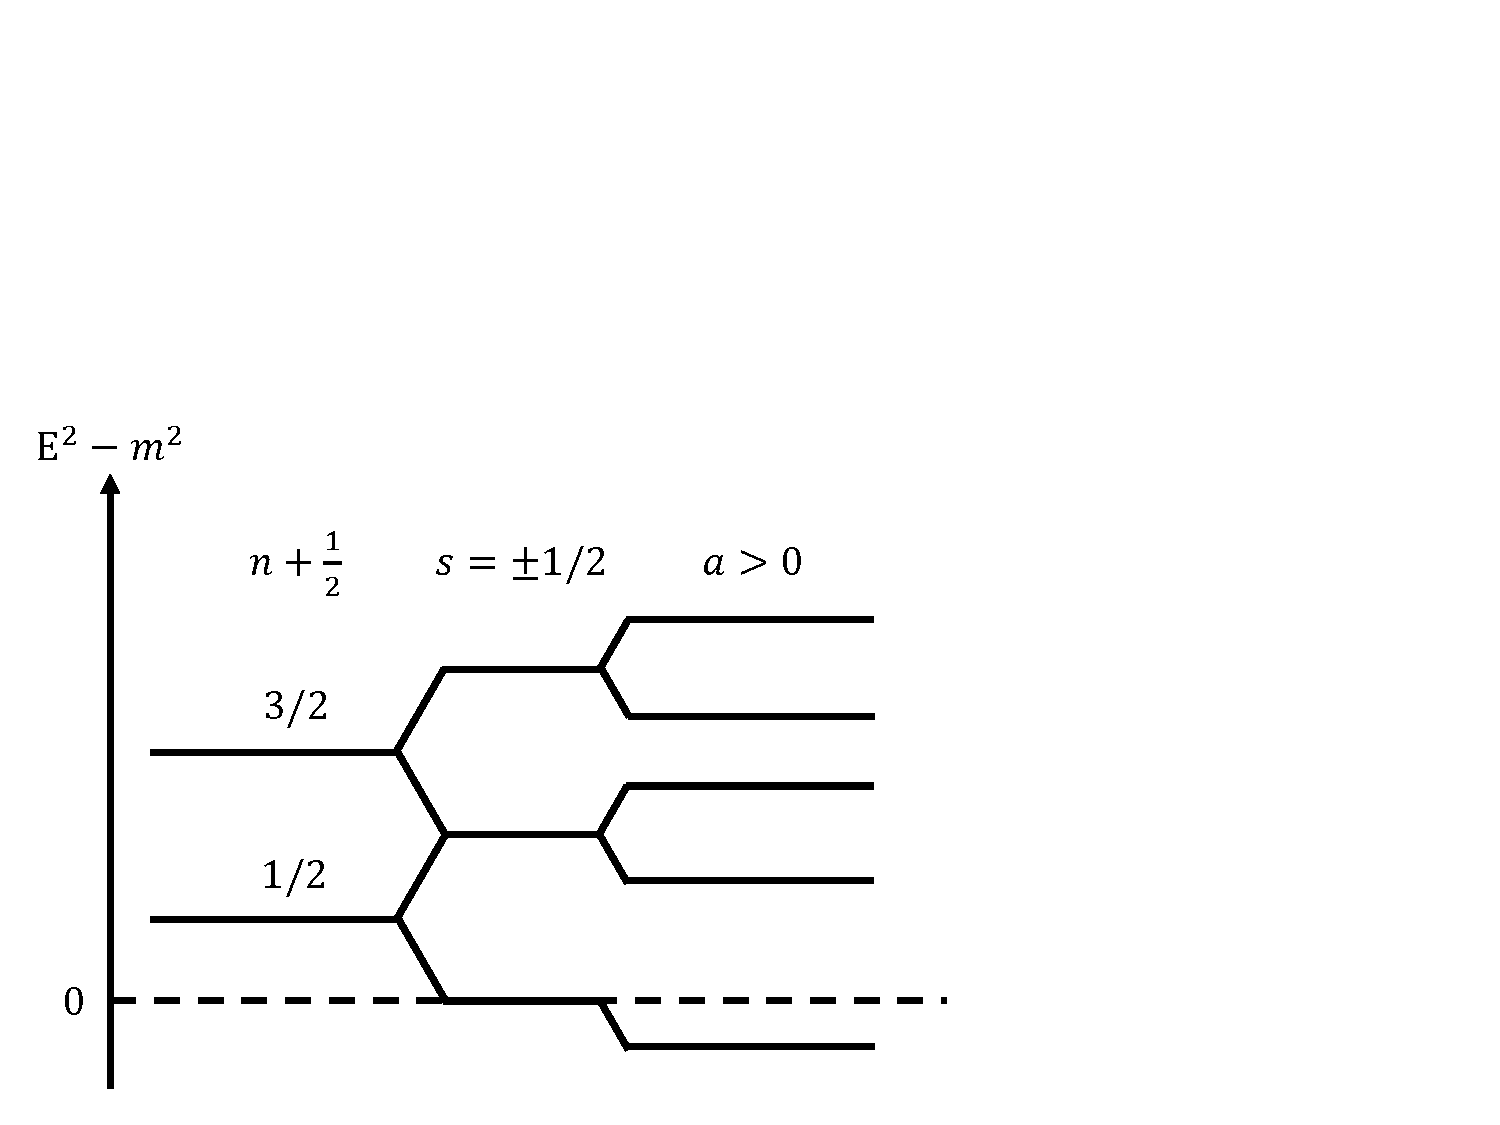
\includegraphics[clip, trim=0.0cm 0.0cm 9.0cm 7.0cm,width=0.6\linewidth]{plots/chap02moment/lanplot04.pdf}
 \caption[]{Diagram organizing the KGP-Landau levels for particles with zero z-component momentum. The Landau levels $n$ and spin $s$ serve to split levels while the anomaly $a$ controls the degeneracy among levels.}
 \label{f04}
\end{figure}
%%%%%%%%%%%%%

However, we recognize a periodicity considering the energy as a function of $g$. We recall that in Eq.~\eqref{lan24b} $n=0, 1, 2\ldots$. As $g$ varies, each time $gs/2$ crosses an integer value, for a different value of $n$ the energy eigenvalue $E$ repeat as a function of changing $g$. All possible values of energy $E$ are reached (at fixed $m$ and $p^2_3$) for $-2\le g\le 2$. Moreover, while for almost all $g\ne 2$ the degeneracy is completely broken, this periodicity implies that energy degeneracy is restored for values~\cite{Evans:2022ygl,Evans:2022fsu} 
\begin{alignat}{1}
\label{lan26}
g_{k}/2=1+k\,,\qquad
\lambda_\mathrm{L}'=\lambda_\mathrm{L}-ks\;,\qquad
\lambda_\mathrm{L}=n+\frac{1}{2}-s\;,
\end{alignat}
where $k=0,\pm1,\pm2,\ldots$ The Landau levels Eq.\,\eqref{lan24} contain an infinite number of degenerate levels bounded from below. Certain states change the sign of the magnetic energy and their total energies become unphysical in the limit that $g_{k}B$ becomes large; for even $k$ there are $k/2$ such states and for odd $k$ there are $(k+1)/2$.

It is useful to compare the KGP solution to the the Landau levels for the DP equation which we obtained by~\cite{Tsai:1971zma}. The DP-Landua energy eigenstates are given by
\begin{subequations}
\begin{alignat}{1}
\label{lan25} 
E^{2}_{n,s}(p_{3},B)|_\mathrm{DP} =&\left(\!\!\sqrt{\displaystyle m_{e}^{2}c^{4}\!+\!2e\hbar c^{2}B\left(n+\frac{1}{2}-s\right)}-\frac{eB\hbar}{2m_{e}}(g-2)s\!\right)^{2}\!\!\!+p_{3}^{\!\!2}c^{2},\\[0.4cm]
\label{lan25b}
E_{n,s}|_\mathrm{DP} =\pm &\sqrt{\!\left(\!\!\sqrt{\displaystyle m_{e}^{2}c^{4}+2e\hbar c^{2}B\left(n+\frac{1}{2}-s\right)}\!-\!\frac{eB\hbar}{2m_{e}}(g-2)s\!\right)^{\!\!2}\!\!\!+p_{3}^{2}c^{2}}\;,
\end{alignat}
\end{subequations}
which in our opinion fails Dirac\rq s principle of mathematical beauty when compared to the KGP result Eq.~\eqref{lan24b}. Both Eqs.~\eqref{lan24b} and \eqref{lan25b} have the correct non-relativistic reduction at the lowest order though, the latter obscures the physical interpretation.

The most egregious issue with the DP-Landau levels is that, in a perturbative expansion, it includes cross terms between the $g\!=\!2$ magnetic moment and anomalous terms in $a=(g-2)/2$; thus the result does not depend on the particle magnetic moment alone; there is a functional dependence on the magnetic anomaly $a$. The presence of these cross terms implies that above first order the results cannot be given in terms of the full magnetic moment alone. In comparison, for the KGP-Landau levels Eq.\,\eqref{lan25b}, the entire effect of magnetic moment is contained in a single term.

%%%%%%%%%%%%%%%%%%%%%%%%%%%%%%%%%%%%%%%
\section{Hydrogen-like atoms}
\label{sec:coulomb}
%%%%%%%%%%%%%%%%%%%%%%%%%%%%%
The Coulomb problem, or sometimes referred to as the Kepler problem, provides us an important application of any quantum theory to explore. As the hydrogen-like atoms are the the most well understood atomic system in physics, any non-minimal behavior especially for high-$Z$ systems can lead to consequences for the resulting spectral lines. We take the Coulomb potential to be
\begin{equation}
	\label{eq:coulomb:01} eV_\mathrm{C}\equiv e A^{0}=\frac{Z \alpha\hbar c}{r}\;,\qquad \bb{A}=0\;.
\end{equation}
The KGP-Coulomb problem with arbitrary magnetic moment can be solved analytically and we will briefly sketch out the solution and its consequences.

For energy states $\Psi=e^{-iEt/\hbar}\Psi_\mathrm{E}$ the KGP equation yields the following differential equation
\begin{alignat}{1}
	\label{cou02} \left(\frac{E^{2}-m^{2}c^{4}}{\hbar^{2}c^{2}}+\frac{Z^{2}\alpha^{2}}{r^{2}}+\frac{2E}{\hbar c}\frac{Z\alpha}{r}+\frac{1}{r}\frac{\partial\bb{L}^{2}}{\partial r^{2}}r-\frac{\bb{L}^{2}/\hbar^{2}}{r^{2}}-\frac{g}{2}Z\alpha\frac{i\bb{\alpha}\cdot\bb{\hat{r}}}{r^{2}}\right)\Psi_\mathrm{E}=0\;.
\end{alignat}
We recast the squared angular momentum operator $\bb{L}^{2}$ with the Dirac spin-alignment operator
\begin{alignat}{1}
\label{cou04} &\mathcal{K}=\gamma^{0}\left(1+\bb{\Sigma}\cdot\frac{\bb{L}}{\hbar}\right)\;,\indent \bb{L}^{2}/\hbar^{2}=\mathcal{K}\left(\mathcal{K}-\gamma^{0}\right)\;.
\end{alignat}
The operator $\mathcal{K}$ commutes with $\bb{\alpha}\cdot\bb{\hat{r}}$ and its eigenvalues are given as either positive or negative integers $\kappa=\pm(j+1/2)$ where $j$ is the total angular momentum quantum number. By grouping all terms proportional to $1/r^{2}$, we see the effective angular momentum eigenvalues take on non-integer values which in the limit of classical mechanics corresponds to orbits which do not close. The non-integer eigenvalues depends explicitly on $g$-factor.

The difficulty of this equation is that the effective angular momentum operator is non-diagonal in spinor space due to the presence of $\bb{\alpha}\cdot\bb{\hat{r}}$ which mixes upper and lower components. The effective radial potential within \req{cou02} is then
\begin{alignat}{1}
	\label{temp} \boxed{V_\mathrm{eff}=-\frac{2E}{\hbar c}\frac{Z\alpha}{r}-\frac{Z^{2}\alpha^{2}}{r^{2}}+\frac{g}{2}Z\alpha\frac{i\bb{\alpha}\cdot\bb{\hat{r}}}{r^{2}}}\,.
\end{alignat}
We emphasize that the distinguishing characteristic which separates the KGP solutions (and Dirac for $g\!=\!2$) from the Klein-Gordon solutions is the last term in the effective potential \req{temp}. This is the dipole-charge interaction term which exists only because of the relativistic expression for the magnetic dipole and is entirely absent non-relativistically. 

Following the procedure of~\cite{Martin:1958zz}, we introduce the operator
\begin{alignat}{1}
\label{cou07} &\mathfrak{L}=-\gamma^{0}\mathcal{K}-\frac{g}{2}Z\alpha(i\bb{\alpha}\cdot\bb{\hat{r}})\;,
\end{alignat}
but with the novel modification that $g$-factor directly appears in the second term. This operator is also sometimes referred to as the Temple operator, therefore we will refer to it as the $g$-Temple operator. This operator then commutes with the spin-alignment operator $\mathcal{K}$ and has eigenvalues
\begin{alignat}{1}
\label{cou08} &\Lambda=\pm\sqrt{\kappa^{2}-\displaystyle\frac{\displaystyle g^{2}}{4}Z^{2}\alpha^{2}}\;,\end{alignat}
where the absolute values are denoted as $\lambda=|\Lambda|$. The angular momentum contributions to \req{cou02} can then be replaced by
\begin{alignat}{1}
\label{cou09} &\mathcal{K}(\mathcal{K}-\gamma^{0})-Z^{2}\alpha^{2}-\frac{g}{2}Z\alpha(i\bb{\alpha}\cdot\bb{\hat{r}})=\mathfrak{L}(\mathfrak{L}+1)+\left(\frac{g^{2}}{4}-1\right)Z^{2}\alpha^{2}.
\end{alignat}
If the $g$-factor is taken to be $g\!=\!2$, then the differential \req{cou02} reverts to the one discussed in~\cite{Martin:1958zz}. The coefficient $g^{2}/4-1$ will be commonly seen to precede new more complicated terms, which conveniently vanish for $|g|=2$ demonstrating that as function of $g$ there is a \lq\lq cusp\rq\rq~\citep{Rafelski:2022bsv} for $|g|=2$. This will become especially evident when we discuss strongly bound systems which behave very differently for $|g|<2$ versus $|g|>2$. 

We omit further derivation which can be found in~\cite{Steinmetz:2018ryf}. We find the resulting energy levels of the KGP-Coulomb equation to be 
\begin{gather}
\label{cou17} E_{\pm\lambda}^{n_{r},j}=mc^{2}\left[1+\displaystyle\frac{Z^{2}\alpha^{2}}{\left(n_{r}+1/2+\nu\right)^{2}}\right]^{-1/2}\,,\\
\label{cou17b} \nu=\sqrt{(\lambda\pm1/2)^{2}+\left(\frac{g^{2}}{4}-1\right)Z^{2}\alpha^{2}}\,,\qquad
\lambda=\sqrt{\displaystyle(j+1/2)^{2}-\frac{\displaystyle g^{2}}{4}Z^{2}\alpha^{2}}\;.
\end{gather}
where $n_{r}$ is the node quantum number which takes on the values $n_{r}=0,1,2,\ldots$. \req{cou17} is the same \lq\lq Sommerfeld-style\rq\rq\ expression for energy that we can obtain from the Dirac or KG equations. The difference between them arises from the expression of the relativistic angular momentum which depends on $g$-factor for the KGP equation. The KGP eigenvalues \req{cou17} for arbitrary spin were obtained by~\cite{Niederle:2004bx} using a tensor approach.

In the limit that $g\rightarrow2$ for the Dirac case the expressions for $\lambda$ and $\nu$ reduce to
\begin{subequations}
\begin{alignat}{1}
\label{glimit01} &\lim_{g\rightarrow2}\lambda=\sqrt{\displaystyle(j+1/2)^{2}-Z^{2}\alpha^{2}},\\
&\lim_{g\rightarrow2}\nu_{\pm\lambda}=\lambda\pm1/2\;.
\end{alignat}
\end{subequations}
This procedure requires taking the root of perfect squares; therefore, the sign information is lost in \req{glimit01}. As long as $Z^{2}\alpha^{2}<3/4$ we can drop the absolute value notation as $\nu$ is always positive. The energy is then given by
\begin{alignat}{1}
\label{glimit02}
E_{\pm\lambda}^{n_{r},j}=mc^{2}\left[1+\displaystyle\frac{Z^{2}\alpha^{2}}{\left(n_{r}\begin{smallmatrix} +1 \\ +0 \end{smallmatrix}+\sqrt{\displaystyle(j+1/2)^{2}-Z^{2}\alpha^{2}}\right)^{2}}\right]^{-1/2}\;.
\end{alignat}
The $\begin{smallmatrix} +1 \\ +0 \end{smallmatrix}$ notation is read as the upper value corresponding to the $+\lambda$ states and the lower value corresponding to the $-\lambda$ states. 

The ground state energy (with: $n_{r}=0,\ \Lambda<0,\ j=1/2$) is therefore
\begin{alignat}{1}
\label{glimit07} &E^{0,1/2}_{-\lambda(j=1/2)}=mc^{2}\sqrt{1-Z^{2}\alpha^{2}}\;,\end{alignat}
as expected for the Dirac-Coulomb ground state. \req{glimit02} reproduces the Dirac-Coulomb energies and also contains a degeneracy between states of opposite $\lambda$ sign, same $j$ quantum number and node quantum numbers offset by one
\begin{alignat}{1}
\label{glimit03} &E^{n_{r}+1,j}_{-\lambda}=E^{n_{r},j}_{+\lambda}\;,\end{alignat}
which corresponds to the degeneracy between $2S_{1/2}$ and $2P_{1/2}$ states. There is no degeneracy for the $E^{0,j}_{-\lambda}$ states. 

In the limit that $g\rightarrow 0$, which is the KG case, the expressions are given by
\begin{subequations}
\begin{alignat}{1}
\label{glimit04} &\lim_{g\rightarrow0}\lambda=j+1/2,\\
&\lim_{g\rightarrow0}\nu_{\pm\lambda}=\sqrt{\left(j\begin{smallmatrix} +1 \\ +0 \end{smallmatrix}\right)^{2}-Z^{2}\alpha^{2}}\;,
\end{alignat}
\end{subequations}
which reproduces the correct expressions for the energy levels for the Klein-Gordon case 
\begin{alignat}{1}
\label{glimit05} E_{\pm\lambda}^{n_{r},j}=mc^{2}\left[1+\displaystyle\frac{Z^{2}\alpha^{2}}{\left(n_{r}+1/2+\displaystyle\sqrt{\left(j\begin{smallmatrix} +1 \\ +0 \end{smallmatrix}\right)^{2}-Z^{2}\alpha^{2}}\right)^{2}}\right]^{-1/2}\;,
\end{alignat}
except that in this limit we are still considering the total angular moment quantum number $j$ rather than orbital momentum quantum number $\ell$. It is interesting to note that the KG-Coulomb problem\rq s energy formula contains $\ell+1/2$, which matches identically to our half-integer $j$ values; therefore, this artifact of spin, untethered and invisible by the lack of magnetic moment, does not alter the energies of the states. The degeneracy in energy levels are given by 
\begin{alignat}{1}
\label{glimit06} &E^{n_{r},j+1}_{-\lambda}=E^{n_{r},j}_{+\lambda}\;,\end{alignat}
with levels of opposite $\lambda$ sign, same node quantum number and shifted $j$ values by one. In a similar fashion to the Dirac case, here we have no degeneracy for $E^{n_{r},1/2}_{-\lambda}$ states.

%%%%%%%%%%%%%%%%%%%%%%%%%%
\subsection{Non-relativistic Coulomb problem energies} \label{nonrel}
The first regime of interest to understand the effect of variable $g$ in the KGP-Coulomb problem is the non-relativistic limit characterized by the weak binding of low-Z atoms. We now will convert from $n_{r}$, $j$ and $\pm\lambda$ to the familiar quantum numbers of $n$, $j$ and $\ell$ allowing for easy comparison with the hydrogen spectrum in standard notation. We start by expanding \req{cou17} in powers of $Z\alpha$ to compare to the known hydrogen spectrum. 

To order $\mathcal{O}(Z^{4}\alpha^{4})$ the energy levels are given by
\begin{alignat}{1}
\label{nonrel01} \frac{E^{n_{r},j}_{\pm\lambda}}{mc^{2}}=1&-\frac{1}{2}\frac{Z^{2}\alpha^{2}}{(n_{r}+1/2+(\nu_{\pm\lambda})|_{Z=0})^{2}}+\frac{(\nu_{\pm\lambda})|_{Z=0}'Z^{3}\alpha^{3}}{(n_{r}+1/2+(\nu_{\pm\lambda})|_{Z=0})^{3}}\\ 
\notag&+\frac{1}{2}\frac{(3/4-3(\nu_{\pm\lambda})|_{Z=0}'^{2})Z^{4}\alpha^{4}}{(n_{r}+1/2+(\nu_{\pm\lambda})|_{Z=0})^{4}}+\frac{1}{2}\frac{(\nu_{\pm\lambda})|_{Z=0}^{\prime\prime} Z^{4}\alpha^{4}}{(n_{r}+1/2+(\nu_{\pm\lambda})|_{Z=0})^{3}}+\mathcal{O}(Z^{6}\alpha^{6})\;,\end{alignat}
where primed $\nu_{\pm\lambda}$ indicate derivatives with respect to $Z\alpha$. These derivatives evaluate to
\begin{alignat}{1}
\label{nonrel02} &(\nu_{\pm\lambda})|_{Z=0}=j+1/2\pm1/2,\\ \notag &(\nu_{\pm\lambda})|_{Z=0}'=0,\\ \notag &(\nu_{\pm\lambda})|_{Z=0}^{\prime\prime}=\frac{(g^{2}/4-1)}{j+1/2\pm1/2}-\frac{g^{2}/4}{j+1/2}\;.
\end{alignat}
\req{nonrel01} then simplifies to
\begin{alignat}{1}
\label{nonrel03} \frac{E^{n_{r},j}_{\pm\lambda}}{mc^{2}}=1&-\frac{1}{2}\frac{Z^{2}\alpha^{2}}{\left(n_{r}+j\begin{smallmatrix}+3/2 \\ +1/2\end{smallmatrix}\right)^{2}}+\frac{3}{8}\frac{Z^{4}\alpha^{4}}{\left(n_{r}+j\begin{smallmatrix}+3/2 \\ +1/2\end{smallmatrix}\right)^{4}}\\ 
\notag &+\frac{1}{2}\left(\frac{(g^{2}/4-1)}{j\begin{smallmatrix}+1 \\ +0\end{smallmatrix}}-\frac{g^{2}/4}{j+1/2}\right)\frac{Z^{4}\alpha^{4}}{\left(n_{r}+j\begin{smallmatrix}+3/2 \\ +1/2\end{smallmatrix}\right)^{3}}+\mathcal{O}(Z^{6}\alpha^{6})\;.
\end{alignat}
In the non relativistic limit, the node quantum number corresponds to the principle quantum number via $n_{r}=n'-j-1/2$ with $n'=1,2,3\ldots$ Using \req{nonrel03} and \req{cou07} we see that in the non relativistic limit $+\lambda$ corresponds to $\kappa>0$ or anti-aligned spin-angular momentum with $j=\ell-1/2$ and $\ell\geq1$. Conversely $-\lambda$ corresponds to $\kappa<0$ or aligned spin-angular momentum with $j=\ell+1/2$. 

With all this input we arrive at
\begin{alignat}{1}
\label{nonrel04} \frac{E^{n,j}_{\begin{smallmatrix}
\kappa>0 \\ \kappa<0
\end{smallmatrix}}}{mc^{2}}=1&-\frac{1}{2}\frac{Z^{2}\alpha^{2}}{\left(n'\begin{smallmatrix}
+1 \\ +0
\end{smallmatrix}\right)^{2}}+\frac{3}{8}\frac{Z^{4}\alpha^{4}}{\left(n'\begin{smallmatrix}
+1 \\ +0
\end{smallmatrix}\right)^{4}}
\\ \notag &+\frac{1}{2}
\frac{(g^{2}/4-1)}{j\begin{smallmatrix}
+1 \\ +0
\end{smallmatrix}}\frac{Z^{4}\alpha^{4}}{\left(n'\begin{smallmatrix}
+1 \\ +0
\end{smallmatrix}\right)^{3}}-\frac{1}{2}\frac{g^{2}/4}{j+1/2}\frac{Z^{4}\alpha^{4}}{\left(n'\begin{smallmatrix}
+1 \\ +0
\end{smallmatrix}\right)^{3}}+\mathcal{O}(Z^{6}\alpha^{6})\;.
\end{alignat}
Lastly we recast, for the $\kappa>0$ states, the principle quantum number as $n'+1\rightarrow n$ with $n\geq2$ and we simply relabel $n'\rightarrow n$ for $\kappa<0$ states. This allows \req{nonrel04} to be completely written in terms of $n$, $j$, and $\ell$ as
\begin{alignat}{1}
\label{nonrel09} \frac{E^{n,j}_{\ell}}{mc^{2}}=1&-\frac{1}{2}\frac{Z^{2}\alpha^{2}}{n^{2}}+\frac{3}{8}\frac{Z^{4}\alpha^{4}}{n^{4}}\\
\notag &+\frac{1}{2}\frac{(g^{2}/4-1)}{\ell+1/2}\frac{Z^{4}\alpha^{4}}{n^{3}}-\frac{1}{2}\frac{g^{2}/4}{j+1/2}\frac{Z^{4}\alpha^{4}}{n^{3}}+\mathcal{O}(Z^{6}\alpha^{6})\;,\end{alignat}
where it is understood that $n-\ell\geq1$, this condition allows us to write what was previously described in \req{nonrel04} as two distinct spectra now as a single energy spectra. In the limit $g\rightarrow2$ or $g\rightarrow0$ the correct expansion to order $Z^{4}\alpha^4$ of the Dirac or KG energies are obtained. In the following we explore some consequences of our principal non-relativistic result, \req{nonrel09}.

%%%%%%%%%%%%%%%%%%%%%%%%%%%%%%
\subsection{g-Lamb Shift between 2S and 2P orbitals} \label{lamb}
The breaking of degeneracy in \req{nonrel09} between states of differing $\ell$ orbital quantum number, but the same total angular momentum $j$ and principle quantum number $n$ is responsible for the Lamb shift due to anomalous magnetic moment. The only term in \req{nonrel09} (up to order $Z^{4}\alpha^{4}$) that breaks the degeneracy between the $E^{n,j}_{\ell=j+1/2}$ and $E^{n,j}_{\ell=j-1/2}$ states for $n\geq2$ is the fourth term. This is unsurprising as it depends exclusively on quantum number $\ell$ and $n$. The lowest order Lamb shift due to anomalous magnetic moment is then
\begin{alignat}{1}
\label{lamb01} \frac{\Delta E_{\mathrm{gLamb}}^{n,j}}{mc^{2}}&=E^{n,j}_{\ell=j-1/2}-E^{n,j}_{\ell=j+1/2}=\left(g^{2}/8-1/2\right)\left(\frac{1}{j}-\frac{1}{j+1}\right)\frac{Z^{4}\alpha^{4}}{n^{3}}\;.
\end{alignat}
For the $2S_{1/2}$ and $2P_{1/2}$ states \req{lamb01} reduces to
\begin{alignat}{1}
\label{lamb02} \frac{\Delta E_{\mathrm{gLamb}}^{2S_{1/2}-2P_{1/2}}}{mc^{2}}&=\left(g^{2}/8-1/2\right)\frac{Z^{4}\alpha^{4}}{6}=\left(a+a^{2}/2\right)\frac{Z^{4}\alpha^{4}}{6}\;.
\end{alignat}
Our result in \req{lamb01} and \req{lamb02} is sensitive to $g^{2}/8-1/2=a+a^{2}/2$. Traditionally the Lamb shift due to an anomalous lepton magnetic moment is obtained perturbatively~\citep{Itzykson:1980rh} by considering the DP equation which is sensitive to $g/2-1=a$ the shift takes on the expression at lowest order
\begin{alignat}{1}
\label{lamb03} \frac{\Delta E_{\mathrm{gLamb,DP}}^{2S_{1/2}-2P_{1/2}}}{mc^{2}}&=\left(\frac{g-2}{2}\right)\frac{Z^{4}\alpha^{4}}{6}=a\frac{Z^{4}\alpha^{4}}{6}\;.
\end{alignat}
It is of experimental interest to resolve this discrepancy between the first order DP equation and the second order fermion formulation KGP. We recall the present day values
\begin{subequations}
\begin{alignat}{1}
\label{aeFULL} a_e&=1159.65218091(26)\times 10^{-6}\simeq \frac{\alpha}{2\pi}\;,\\
a_\mu-a_e&=6.2687(6)\times 10^{-6}\;.
\end{alignat}
\end{subequations}
The largest contribution to the anomalous moment for charged leptons is, as indicated the lowest order QED Schwinger result $a=\alpha/2\pi$. For the KGP approach, the anomalous $g$-factor mixes contributions of different powers of fine structure $\alpha$. Precision values for the fundamental constants are taken from~\cite{Tiesinga:2021myr}. For the $2S_{1/2}-2P_{1/2}$ states, the shift is
\begin{alignat}{1}
\label{lamb04} &\frac{\Delta E_{\mathrm{gLamb}}^{2S_{1/2}-2P_{1/2}}}{mc^{2}}=\frac{Z^{4}\alpha^{5}}{12\pi}+\frac{Z^{4}\alpha^{6}}{48\pi^{2}}\;.
\end{alignat}
The scale of the discrepancy between KGP and DP for the hydrogen atom is then
\begin{alignat}{1}
\label{lamb05} \Delta &E_{\mathrm{gLamb,KGP}}^{2S_{1/2}-2P_{1/2}}\!-\!\Delta E_{\mathrm{gLamb,DP}}^{2S_{1/2}-2P_{1/2}}\!=\!\frac{\alpha^{6}mc^{2}}{48\pi^{2}}\\ \notag&\;\;=\!1.62881214\times10^{-10}\;\mathrm{eV} =39.3845030\;\mathrm{kHz}\;,\end{alignat}
without taking into account the standard corrections such as reduced mass, recoil, radiative, or finite nuclear size; for more information on those corrections please refer to~\cite{Tiesinga:2021myr,Jentschura:1996zz,Eides:2000xc}. It is to be understood that the corrections presented here are illustrative of the effect magnetic moment has on the spectroscopic levels, but that further work is required to compare these to experiment: for example we look here on behavior of point particles only.

While the discrepancy is small for the hydrogen system, it is $\approx 40$ kHz and will be visible in this or next generation\rq s spectroscopic experiments. The discrepancy is also non-negligible for hydrogen-like exotics such as proton-antiproton because the proton $g$-factor is much larger
\begin{alignat}{1}\label{gpaFULL}
&g_p=5.585694702(17)\;,\qquad a_p=1.792847351(9)\;. 
\end{alignat} 
The discrepancy for the proton-antiproton system is
\begin{alignat}{1}
\label{lamb06} \Delta E_{\mathrm{gLamb,KGP}}^{2S_{1/2}-2P_{1/2}}-\Delta E_{\mathrm{gLamb,DP}}^{2S_{1/2}-2P_{1/2}}&=0.71268151\;\mathrm{eV}\;.
\end{alignat} 

%%%%%%%%%%%%%%%%%%%%%%%
\subsection{g-Fine structure effects within P orbitals} \label{fs}
The fifth term in \req{nonrel09}, which depends on $j$ and $n$, will shift the levels due to an anomalous moment, but does not contribute to the Lamb shift. Rather this expression, which contains the spin-orbit $\vec{L}\cdot\vec{S}$ coupling, is responsible for the fine structure splittings. From \req{nonrel09} the fine structure splitting is given by
\begin{alignat}{1}
\label{fs00} \frac{\Delta E_{\mathrm{gFS}}^{n,\ell}}{mc^{2}}&=E^{n,j=\ell+1/2}_{\ell}-E^{n,j=\ell-1/2}_{\ell}=\left(g^{2}/8\right)\left(\frac{1}{\ell}-\frac{1}{\ell+1}\right)\frac{Z^{4}\alpha^{4}}{n^{3}}\;.
\end{alignat}
The splitting between the $2P_{3/2}$ and $2P_{1/2}$ states is therefore
\begin{alignat}{1}
\label{fs01} \frac{\Delta E_{\mathrm{gFS}}^{2P_{3/2}-2P_{1/2}}}{mc^{2}}&=\left(g^{2}/8\right)\frac{Z^{4}\alpha^{4}}{16}=\left(1/2+a+a^{2}/2\right)\frac{Z^{4}\alpha^{4}}{16}\;.
\end{alignat}
In comparison the fine structure dependence on $g$-factor in the DP equation is given as
\begin{alignat}{1}
\label{fs02} \frac{\Delta E_{\mathrm{gFS,DP}}^{2P_{3/2}-2P_{1/2}}}{mc^{2}}&=\left(\frac{g-1}{2}\right)\frac{Z^{4}\alpha^{4}}{16}=\left(1/2+a\right)\frac{Z^{4}\alpha^{4}}{16}\;.
\end{alignat}
Just as in the case of the Lamb shift, we find that the KGP and DP equations disagree for fine structure splitting. For the hydrogen atom this discrepancy is 
\begin{alignat}{1}
\label{fs03} \Delta &E_{\mathrm{gFS,KGP}}^{2P_{3/2}-2P_{1/2}}\!-\!\Delta E_{\mathrm{gFS,DP}}^{2P_{3/2}-2P_{1/2}}\!=\!\frac{\alpha^{6}mc^{2}}{128\pi^{2}}\\ \notag&\;\;=\!6.10804553\times10^{-11}\;\mathrm{eV}=14.7691885\;\mathrm{kHz}\;,\end{alignat}
and for proton-antiproton, the fine structure splitting discrepancy is
\begin{alignat}{1}
\label{fs04} \Delta E_{\mathrm{gFS,KGP}}^{2P_{3/2}-2P_{1/2}}-\Delta E_{\mathrm{gFS,DP}}^{2P_{3/2}-2P_{1/2}}&=0.26725557\;\mathrm{eV}\;.
\end{alignat}
For fine structure of the muonic-hydrogen system, the KGP-DP discrepancy is
\begin{alignat}{1}
\label{fs05} \Delta E_{\mathrm{gFS,KGP}}^{2S_{1/2}-2P_{1/2}}-\Delta E_{\mathrm{gFS,DP}}^{2S_{1/2}-2P_{1/2}}&=\!1.272774\times10^{-8}\;\mathrm{eV}\;
\end{alignat} 
We can make a general observation that non minimal magnetic coupling, such as we have studied in the DP and KGP cases, enlarge energy level splittings. The above shows that these discrepancies will remain when calculating within more realistic finite nuclear size context.

















%%%%%%%%%%%%%%%%%%%%%%%%%%%%%%%%%%%%%%%
\section{Particles in strong electromagnetic fields}
\label{sec:sb}
%%%%%%%%%%%%%%%%%%%%%%%%%%%%%%%%%%%%%%%
Care must be taken when interpreting the results presented in sections. For physical electrons the AMM interaction is the result of vacuum fluctuations whose strength also depends on the strength of the field. For example in the large magnetic field limit a QED computation shows that the ground state is instead of \req{lan24b} given by~\cite{Jancovici:1969exc}
\begin{alignat}{1} \label{vacfl01}
E_{0}\approx mc^{2}+\frac{\alpha}{4\pi}mc^{2}\ \mathrm{ln}^{2}\left(\frac{2e\hbar B}{m^{2}c^{3}}\right)
\end{alignat}
which even for enormous magnetic fields does not deviate significantly from the rest mass-energy of the electron. Further the AMM radiative corrections approach zero for higher Landau levels~\citep{Ferrer:2015wca,Hackebill:2022uxv}. Therefore the AMM in the case of electrons does not have a significant effect in highly magnetized environments such as those found in astrophysics (magnetars).

The situation is different for composite particles such as the proton, neutron and light nuclei whose anomalous magnetic moments are dominated by their internal structure and not by vacuum fluctuations. In this situation we expect that the AMM interaction in high magnetic fields remains significant. Therefore, asking whether the DP or KGP equations better describes the dynamics of composite hadrons and atomic nuclei in presence of magnetar strength fields is a relevant question despite the standard choice in literature being the DP equation~\citep{Broderick:2000pe}. The same question can be asked for certain exotic hydrogen-like atoms where the constituent particles have anomalous moments which can be characterized as an external parameter. 

%%%%%%%%%%%%%%%%%%%%%%%%%%%%%%%%%%%%%%%
\subsection{Strong homogeneous magnetic fields}
\label{sec:sbl}
%%%%%%%%%%%%%%%%%%%%%%%%%%%%%%%%%%%%%%%
\noindent The magnetic moment anomaly can flip the sign of the magnetic energy for the least excited states causing the gap between particle and antiparticle states to decrease with magnetic field strength. Setting $p_z=0$ in \req{lan24}, we show in figure~\ref{f01} that the energy of the lowest KGP Landau eigenstate $n=0, s=1/2$ reaches zero where the gap between particle and antiparticle states vanishes for the field
\begin{subequations}
\begin{alignat}{1}\label{Bcrit}
&B_\mathrm{crit}^{e}=\frac{{B}_{S}^{e}}{a_{e}}\simeq861{B}_{S}^{e} =3.8006\times10^{16}\;\mathrm{G}\;,\\
&B_\mathrm{crit}^{p}=\frac{{B}_{S}^{p}}{a_{p}}\simeq\frac{1}{1.79}{B}_{S}^{p}=8.3138\times10^{19}\;\mathrm{G}\;,
\end{alignat} 
\end{subequations}
where ${B}_{S}$ is the so-called Schwinger critical field~\citep{Schwinger:1951nm}.
\begin{subequations}
\begin{alignat}{1}\label{Bsch}
{B}_{S}^{e}\equiv\frac{{m_{e}^2}c^2}{e\hbar}=\frac{m_{e}c^2}{2\mu_B}=4.4141\times 10^{13}\;\mathrm{G}\;,\\
{B}_{S}^{p}\equiv\frac{{m_{p}^2}c^2}{e\hbar}=\frac{m_{p}c^2}{2\mu_N}=1.4882\times 10^{20}\;\mathrm{G}\;.
\end{alignat}
\end{subequations}
The numerical results are evaluated for the anomalous moment of the electron and proton, given by \req{aeFULL} and \req{gpaFULL}. At the critical field strength $B_\mathrm{crit}$ the Hamiltonian loses self-adjointness and the KGP loses its predictive properties. The Schwinger critical field \req{Bsch} denotes the boundary when electrodynamics is expected to behave in an intrinsically nonlinear fashion, and the equivalent electric field configurations become unstable~\citep{Labun:2008re}. However, it is also possible that the vacuum is stabilized by such strong magnetic fields~\citep{Evans:2018kor}.
 
%%%%%%%%%%%%%%%%%%%%%%%%%%%%%%%%%%%%%%%
\begin{figure}[h]
     \centering
     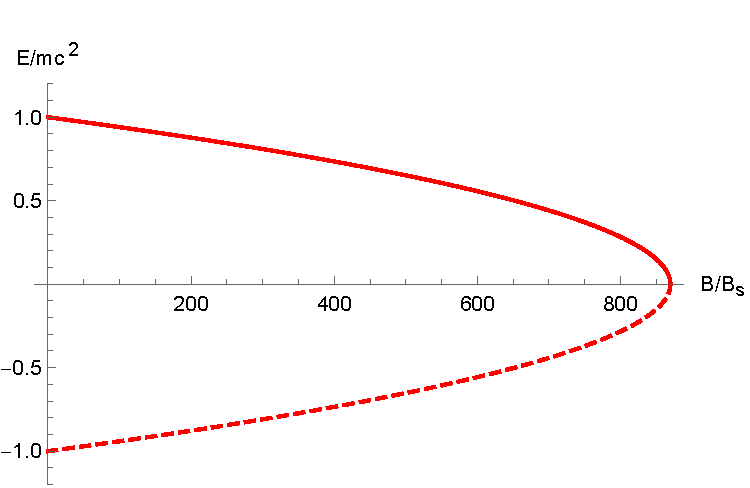
\includegraphics[clip, trim=0.0cm 0.0cm 0.0cm 0.5cm,width=0.95\textwidth]{plots/chap02moment/lanplot01.pdf}
     \caption{The $n=0$, $s=1/2$ ground state for a KGP electron given by \req{lan24b} with $g/2-1=\alpha/2\pi$ in a homogeneous magnetic field. We consider the particle with no $z$-direction momentum. The particle state (solid red) and antiparticle (dashed red) are presented.}
     \label{f01}
\end{figure}
%%%%%%%%%%%%%%%%%%%%%%%%%%%%%%%%%%%%%%%

The critical magnetic fields as shown in \req{Bcrit} appear in discussion of magnetars~\citep{Kaspi:2017fwg}. The magnetar field is expected to be more than 100-fold that of the Schwinger critical magnetic field which is on the same order of magnitude as $B_\textrm{crit}$ for an electron. While the critical field for a proton exceeds that of a magnetar, the dynamics of protons (and neutrons) in such fields is nevertheless significantly modified. A correct description of magnetic moment therefore has relevant consequences to astrophysics. 

Figure~\ref{f02} shows analogous reduction in particle/anti\-particle energy gap for the DP equation. In this case the vanishing point happens at a larger magnetic field strength. This time the solutions continue past this point, but require allowing the states to cross into the opposite continua which we consider unphysical. We are not satisfied with either model\rq s behavior though the KGP description is preferable. However, it is undesirable that both KGP and DP solutions loose physical meaning and vacuum stability in strong magnetic fields.

%%%%%%%%%%%%%%%%%%%%%%%%%%%%%%%%%%%%%%%
\begin{figure}[h]
     \centering
     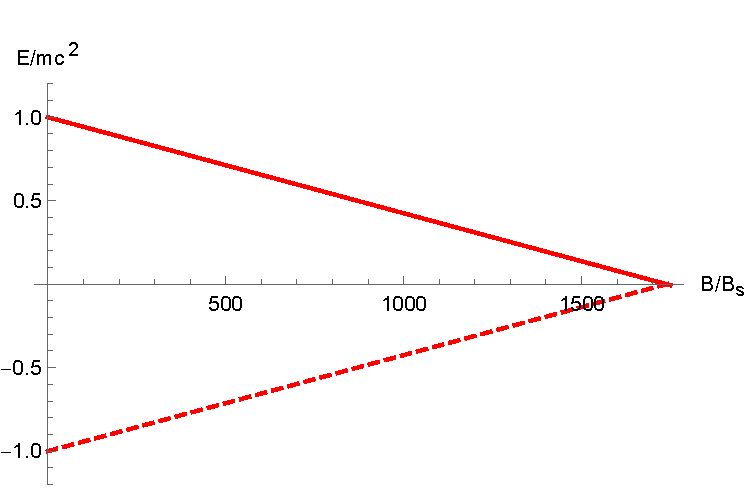
\includegraphics[clip, trim=0.0cm 0.0cm 0.0cm 0.5cm,width=0.95\textwidth]{plots/chap02moment/lanplot02.pdf}
     \caption{The $n=0$, $s=1/2$ ground state for a DP electron given by \req{lan25b} with $g/2-1=\alpha/2\pi$ in a homogeneous magnetic field. We consider the particle with no $z$-direction momentum. The particle state (solid red) and antiparticle (dashed red) are presented.}
     \label{f02}
\end{figure}
%%%%%%%%%%%%%%%%%%%%%%%%%%%%%%%%%%%%%%%

%%%%%%%%%%%%%%%%%%%%%%%%%%%%%%%%%%%%%%%
\subsection{High-Z hydrogen-like atoms}
\label{sec:sbc}
%%%%%%%%%%%%%%%%%%%%%%%%%%%%%%%%%%%%%%%
\noindent For the case of $g\!=\!2$ hydrogen-like systems with large $Z$ nuclei, there is extensive background related to the long study of the solutions of the Dirac equation~\citep{Rafelski:1976ts,Greiner:1985ce,Rafelski:2016ixr}. For $g\ne 2$ and $1/r$ singular potential we refer back to the exact expression for the energy levels in \req{cou17}. In the situation of critical electric fields, states lose self-adjointness for large $Z$. For $|g|<2$, just as in the Dirac energy levels for $1/r$ singular potential, but if $|g|>2$ there is merging of particle to particle states (and antiparticle to antiparticle) for states of the same total angular momentum quantum number $j$, but opposite spin orientations.

This behavior can be seen in figure~\ref{f03}, which shows the meeting of the $1S_{1/2}$ and $2P_{1/2}$ states. For $|g|<2$ there is no state merging, but for small anomalies the solution is discontinuous in the sense that even for 1S$_1/2$ we see in figure~\ref{f03} a maximum allowed value of $Z$ at a finite energy. This behavior is reminiscent of the behavior we are familiar with for $1/r$ potential for the 2P$_1/2$ (seen in figure~\ref{f03}) and many other $g\!=\!2$ eigenstates. We know from study of numerical solutions of the Dirac equation that the regularization of the Coulomb potential by a finite nuclear size removes this singular behavior. It remains to be seen how this exactly works in the context of the KGP equation allowing for the magnetic anomaly.

%%%%%%%%%%%%%%%%%%%%%%%%%%%%%%%%%%%%%%%
\begin{figure}[h]
    \centering
    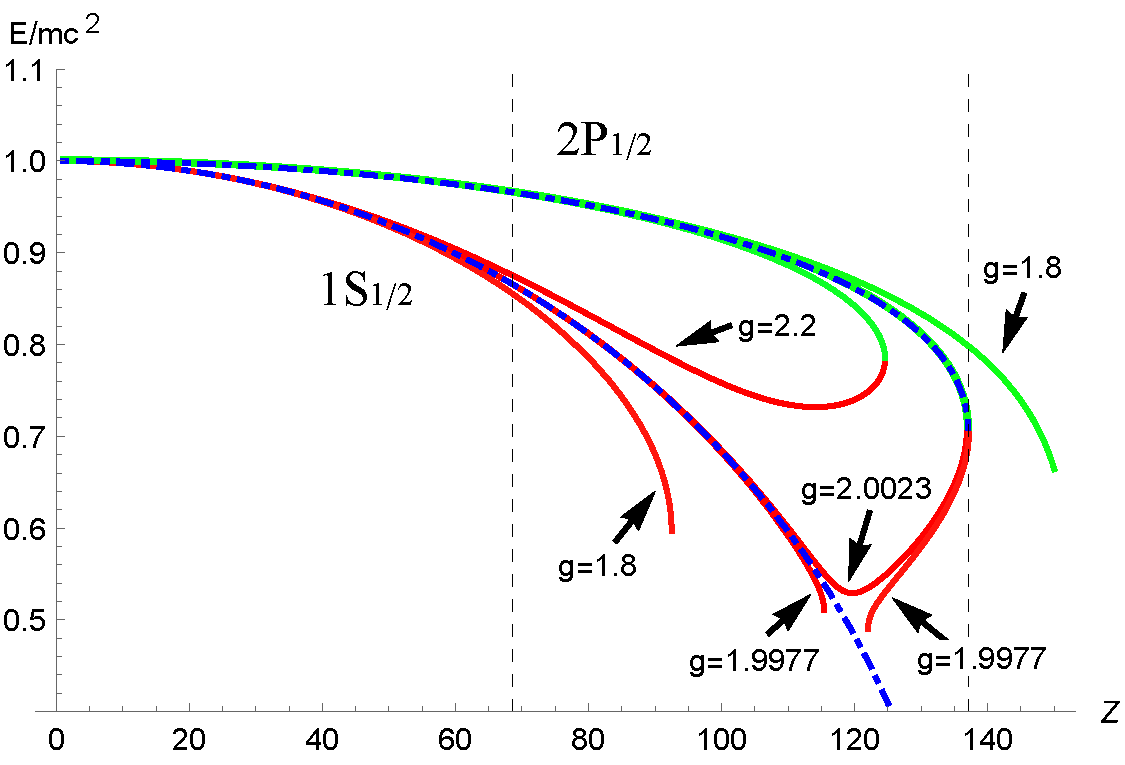
\includegraphics[width=\linewidth]{plots/chap02moment/lanplot08.pdf}
     \caption{The KGP $1S_{1/2}$ (lower red curves) and $2P_{1/2}$ (upper green curves) energy levels for $g$-factor values $g\!=\!\{1.8,\ 1.9977,\ 2.0023,\ 2.2\}$ are shown for large $Z$ hydrogen-like atoms. The curves for the Dirac $g\!=\!2$ case for (lower dashed blue) $1S_{1/2}$ and (upper dashed blue) $2P_{1/2}$ are also presented.}
    \label{f03}
\end{figure}
%%%%%%%%%%%%%%%%%%%%%%%%%%%%%%%%%%%%%%%

The Dirac $g\!=\!2$ case acts as unique \lq\lq cusp\rq\rq\ point because even for very small anomalies, as emphasized in figure~\ref{f03}, the behavior of the states is strongly modified for the situation of high intensity Coulomb fields which are present in large $Z$ hydrogen-like nuclei.

\cite{Thaller:1992ji} presented numerically computed DP equation energy levels for large $Z$ hydrogen like atoms. These numerical solutions involve crossings in energy levels between states with the same total angular quantum number $j$, but differing spin orientations such as $1S_{1/2}$ and $2P_{1/2}$; these states also have the behavior of diving into the antiparticle lower continuum even for $1/r$-potential. These features are not present for the KGP-Coulomb solution. However, there is a similarity between the numerical solutions of the DP equation and our analytical KGP solutions, because for $|g|>2$ the merging states as described above correspond to the crossing states in the DP solution.

The DP equation also allows for the so-called `super-positronium' states as described~\cite{Barut:1975hz,Barut:1976hs}. Such states represent resonances due to the magnetic interaction that reside incredibly close to the center of the atom i.e $\sqrt{\langle r^{2}\rangle}\approx a\alpha\hbar/mc$, but this feature is absent from the KGP formation of the Coulomb problem as all KGP-Coulomb wave functions which can be normalized can be successfully matched to their Dirac ($g\!=\!2$) companions.

%%%%%%%%%%%%%%%%%%%%%%%%%%%%%%%%%%%%%%%
\begin{figure}[h]
    \centering
    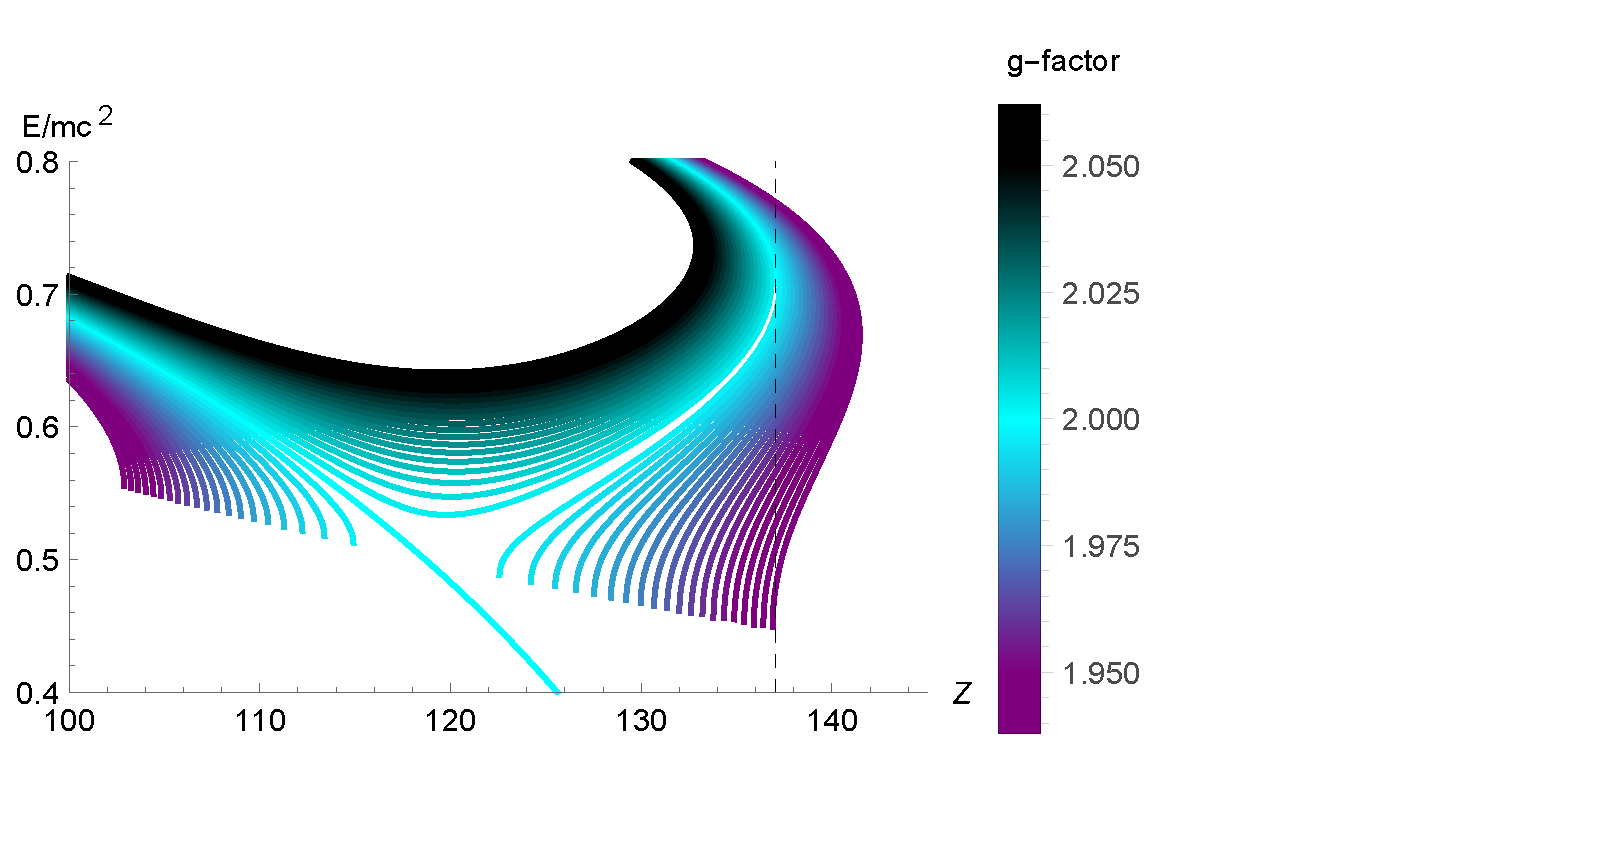
\includegraphics[clip, trim=0.0cm 0.0cm 8.0cm 0.0cm,width=0.95\linewidth]{plots/chap02moment/lanplot05.pdf}
     \caption{Add this bit in!}
    \label{fig:gspec}
\end{figure}
%%%%%%%%%%%%%%%%%%%%%%%%%%%%%%%%%%%%%%%

Because analytical solutions of DP equation, unlike our results for KGP, are not available it is hard to pinpoint precisely the origin of the diverse unpalatable behavior. However, we can hypothesize that the problems arise due to the pathological structure of DP equation where the magnetic anomaly rather than full magnetic moment appears. In any case we see that the Thaller solutions present pathologies quite akin to those we already described in our study of Landau energies. On the other hand KGP framework for large $Z$ shows some exciting and nice analytical behavior.

%%%%%%%%%%%%%%%%%%%%%%%%%%%%%%%%%%%%%%%
\section{Special topics related to Klein-Gordon-Pauli}
\label{sec:kgptopics}
%%%%%%%%%%%%%%%%%%%%%%%%%%%%%%%%%%%%%%%
\subsection{Combination of mass and magnetic moment}
\label{sec:ikgp}
%%%%%%%%%%%%%%%%%%%%%%%%%%%%%%%%%%%%%%%
While we've thus far focused on the Dirac-Pauli and Klein-Gordon-Pauli models for magnetic dipole moments, the non-uniqueness of spin dynamics allows us to invent further non-linear EM models which all in the non-relativistic limit yield the non-relativistic QM magnetic dipole Hamiltonian. One such extension to quantum spin dynamics is to note the close relationship mass and magnetic moment share in the KGP formalism. We can write a unified dipole-mass as
\begin{alignat}{1}
    \label{eq:ext:01} \boxed{\widetilde{m}(\bb{E},\bb{B}) = m +\mu\frac{\sigma_{\alpha\beta}F^{\alpha\beta}}{2c^{2}}}\,,
\end{alignat}
which satisfies the wave equation
\begin{gather}
\label{eq:ext:02} \left((i\hbar\partial_{\mu}-eA_{\mu})^{2}-\widetilde{m}^{2}(\bb{E},\bb{B})c^{2}\right)\Psi=0\,,\\
\label{IKGP01} \left(\left(i\hbar\partial_{\mu}-eA_{\mu}\right)^{2}-\left(mc+\mu\frac{\sigma^{\alpha\beta}F_{\alpha\beta}}{2c}\right)^{2}\right)\Psi=0\;.
\end{gather}
This modified KGP formulation then requires spin sensitive mass and an explicit electromagnetic component to the charged lepton mass. As informed by classical mechanics, charged particles should be understood to derive at least some of their mass from the mass-energy of their electromagnetic fields. \req{quad:1} results in higher order vertex diagrams coupling fermions to photons.

The approach in \req{eq:ext:01} is superficially similar to the model proposed by~\cite{Frenkel:1926zz} in classical mechanics by giving the particle a spin dependent mass of the form $m\sim\Sigma_{\mu\nu}F^{\mu\nu}$ where $\Sigma_{\mu\nu}$ is the covariant generalization of the classical magnetic and electric dipole. \req{IKGP01} is however distinct in that the mass is allowed off-diagonal components in spinor space (a subspace which doesn't exist classically). The dipole-mass \req{eq:ext:01} is off-diagonal in spinor space in the Dirac representation and no longer commutes likes a scalar.

\req{eq:ext:01} also differs from the regular KGP equation by the presence of an additional quadratic interaction which we can evaluate using \req{dp:2} in the Dirac basis as
\begin{gather}
    \label{quad:1} \delta V=-\frac{\mu^{2}}{4}\left(\gamma_{\alpha}\gamma_{\beta}F^{\alpha\beta}\right)^{2}=\mu^{2}
    \begin{pmatrix}
        i\bb{\sigma}\cdot\bb{E}/c & -\bb{\sigma}\cdot\bb{B} \\
        -\bb{\sigma}\cdot\bb{B} & i\bb{\sigma}\cdot\bb{E}/c
    \end{pmatrix}
    \begin{pmatrix}
        i\bb{\sigma}\cdot\bb{E}/c & -\bb{\sigma}\cdot\bb{B} \\
        -\bb{\sigma}\cdot\bb{B} & i\bb{\sigma}\cdot\bb{E}/c
    \end{pmatrix}\,,\\
    \label{quad:2}
    \delta V = \mu^{2}
    \begin{pmatrix}
        \bb{B}^{2}-\bb{E}/c^{2} & -i\bb{E}\cdot\bb{B} \\
        -i\bb{E}\cdot\bb{B} & \bb{B}^{2}-\bb{E}/c^{2}
    \end{pmatrix}=2\mu^{2}
    \begin{pmatrix}
        \mathcal{S} & -i\mathcal{P} \\
        -i\mathcal{P} & \mathcal{S}
    \end{pmatrix}\,.
\end{gather}
We define the invariants of the electromagnetic field tensor $F^{\alpha\beta}$ in \req{quad:2}  letting us write the above more compactly as
\begin{alignat}{1}
    \label{inv:1} \mathcal{S}=\frac{1}{2}(\bb{B}^{2}-\bb{E}^{2}/c^{2})\,,\qquad
    \mathcal{P}=\bb{E}\cdot\bb{B}/c\,,\qquad
    \delta V=2\mu^{2}\left(\mathcal{S}-i\gamma^{5}\mathcal{P}\right)\,.
\end{alignat}
We note that $\sigma_{\alpha\beta}F^{\alpha\beta}/2$ can also be written in terms of its four eigenvalues
\begin{align}
    \label{inv:2}
    \lambda_{1}=+\mathcal{S}+i\mathcal{P}\,,\qquad
    \lambda_{2}=+\mathcal{S}-i\mathcal{P}\,,\qquad
    \lambda_{3}=-\mathcal{S}+i\mathcal{P}\,,\qquad
    \lambda_{4}=-\mathcal{S}-i\mathcal{P}\,.
\end{align}
This represents simply only one possible non-linear extension to electromagnetism in relativistic quantum mechanics of which there are a family of extensions~\citep{Foldy:1952a}.

For the homogeneous magnetic field \req{IKGP01} can be solved in much the same way as the KGP equation in \rsec{sec:homogeneous}. One obtains energy eigenvalues by noting the simple shift that occurs in the mass of $m^2\rightarrow m^{2}+\mu^{2}{B}^{2}$ quadratic in the magnetic field. The resulting energy levels are
\begin{alignat}{1}
\label{IKGP05} E_{n,s}(\bb{B})=\sqrt{m_{e}^{2}c^{4}+\mu^{2}{B}^{2}+p_{3}^{2}c^{2}+2e\hbar c^{2}B\left(n+\frac{1}{2}\right)-2\mu B m_{e}c^{2}s}
\end{alignat}
An interesting feature is that in ultra-high magnetic fields ($B>>{B}_{s}$), Eq.~\eqref{IKGP05} approximates
\begin{alignat}{1}
\label{IKGP07} E\approx\mu B\;.
\end{alignat}
This is not dissimilar to the non-relativistic case where the magnetic energy is simply proportional to the magnetic field.

%%%%%%%%%%%%%%
\begin{figure}[h]
 \centering
 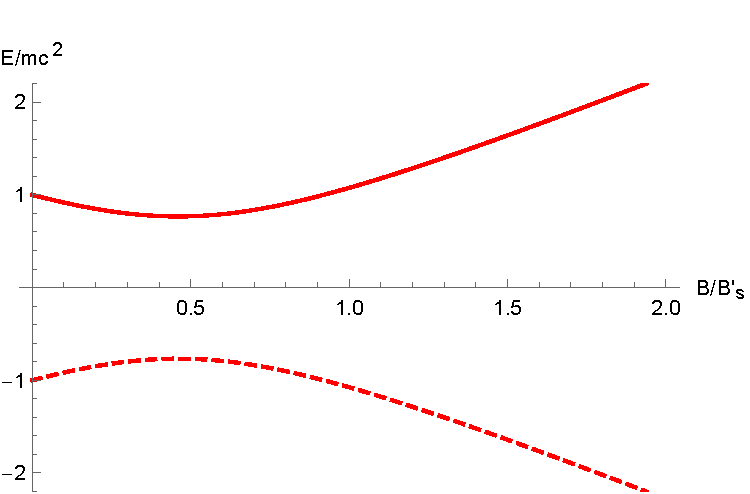
\includegraphics[clip, trim=0.0cm 0.0cm 0.0cm 0.5cm,width=\linewidth]{plots/chap02moment/lanplot09.pdf}
 \caption{The $n=0$, $s=1/2$ ground state for a IKGP proton given by Eq.~\eqref{IKGP05} with $g=5.58$ in a homogeneous magnetic field. The magnetic minimum is well visible for particles with larger anomalous moment such as proton. We consider the particle with no $z$-direction momentum. The particle state (solid red) and antiparticle (dashed red) are presented. The magnetic field scale is ${B}'_{S}=(m^2_p/m^2_e){B}_S$.}
\label{f05}
\end{figure}
%%%%%%%%%%%%%%

The most striking feature is that the ground state remains physical for all values of magnetic field when an anomalous moment is included. The self-adjointness of the system is not lost for some critical magnetic field strength. It can be then thought that the magnetic field provides a stabilizing influence on the system. Rather, there exists a \lq\lq magnetic minimum\rq\rq\ located for $n=0, s=1/2$ at
\begin{alignat}{1}
\label{IKGP06} B_{\mathrm{min}}&=\frac{4mc^{2}}{g^{2}\mu_{B}}a\;,
\end{alignat}
which for the electron is
\begin{alignat}{1}
B_{\mathrm{min}}^{e}&=\frac{8a_e}{g_e^2}{B}_S
=1.02126\times10^{11}\;\mathrm{G}\;.
\end{alignat}
The minimum for a proton is in comparison
\begin{alignat}{1}
B_{\mathrm{min}}^{p}&=\frac{8a_p}{g_p^2} \frac{m_p^2}{m_e^2}{B}_s
=6.841\times10^{19}\;\mathrm{G}\;,
\end{alignat}
which can be seen in~\rf{f05}. Here it is understood that for the calculation of the proton's magnetic minimum, the nuclear mass and magneton was used rather than the electron Bohr magneton. For large enough g-factor, excited states may also contain a minimum, but for any nonzero anomalous moment the ground state always does.

%%%%%%%%%%%%%%%%%%%%%%%%%%%%%%%%%%%%%%%
\subsection{Extensions to non-Albelian fields}
\label{sec:quarks}
%%%%%%%%%%%%%%%%%%%%%%%%%%%%%%%%%%%%%%%

%While most attention in particle physics focuses on the dipole moments of fermions, it is well known that bosons with spin can also carry dipole moments. The most pertinent example is that of the W-boson which after electroweak symmetry breaking has a magnetic dipole term which is analogous to the Pauli term in KGP or DP for fermions. While a wide variety of spin-1 formulations exist, such as the Duffin-Kemmer formulation \ar, in the following discussion we will write in the Proca formulation as it is most similar to how electromagnetic fields, which are also spin-1 fields, are written. For a complex spin-1 field, the Proca action is given by
%\begin{alignat}{1}
%	\label{eq:proca:01a} \mathcal{L}_{\mathrm{Proca}} = -\frac{1}{2}\mathcal{F}_{\mu\nu}^{*}\mathcal{F}^{\mu\nu}+\frac{m^{2}c^{2}}{\hbar^{2}}B_{\mu}^{*}B^{\mu}\,,\\
%	\label{eq:proca:01b} \mathcal{F}^{\mu\nu}=\partial^{\mu}B^{\nu}-\partial^{\nu}B^{\mu}\,.
%\end{alignat}
%The Euler-Lagrangian equations of motion are then
%\begin{alignat}{1}
%	\label{eq:proca:02a} \partial_{\mu}\mathcal{F}^{\mu\nu}+\frac{m^{2}c^{2}}{\hbar^{2}}B^{\nu}=0\,,
%\end{alignat}
%which if the Lorenz gauge $\partial\cdot B=0$ is taken simplifies to a Klein-Gordon style second-order wave equation. If we gauge the fields giving the spin-1 field an electric charge, we can produce a theory which naturally generates a magnetic moment.

Briefly, we would like to comment on the g-factor of the quarks who unlike the leptons also participate in the strong color interaction. Since color charge follows a more complex SU(3) group structure unlike the more straight forward U(1) of electromagnetism, the \lq\lq color magnetism\rq\rq\ of QCD requires more than just the analogous Pauli term to describe color dipole moments owing due to the fact that QCD has non-Abelian gauge fields. The quarks, like the leptons, should obey the quantum mechanical analogue of the energy-momentum relation seen in \req{eq:spin:03} with the only theoretical difference being a differing covariant derivative. The covariant derivative, written in terms of momentum, should appear as
\begin{alignat}{1}
	\label{eq:spin:08} \pi^{\alpha}=p^{\alpha}-g_\mathrm{S}\mathcal{A}^{\alpha}\,,
\end{alignat}
where $g_\mathrm{S}$ is the color charge strength and not to be confused with the QCD notion of g-factor. The gluon fields $\mathcal{A}^{\alpha}$ is a $3\times3$ matrix to accomodate the three charges of QCD: red, green and blue. The eight Gell-Mann $\lambda^{a}$ matrices are embbeded into the gluon field for each possible gluon charge.
\begin{alignat}{1}
	\label{eq:spin:09} \mathcal{A}^{\alpha}\equiv\frac{1}{2}\lambda^{a}\mathcal{A}^{\alpha}_\mathrm{A}\,,\indent a\in1\ldots8\,,
\end{alignat}
We note the non-commuting behavior of the Gell-Mann matrices which capture the non-Abelian structure of the gauge fields. The gluon strength tensor $\mathcal{G}^{\mu\nu}$ is then
\begin{alignat}{1}
	\label{eq:spin:10a} \mathcal{G}^{\mu\nu}\equiv\partial^{\mu}\mathcal{A}^{\nu}-\partial^{\nu}\mathcal{A}^{\mu}+ig_\mathrm{S}\left[\mathcal{A}^{\mu},\mathcal{A}^{\nu}\right]\,,\\
	\label{eq:spin:10b} \left[\mathcal{A}^{\mu},\mathcal{A}^{\nu}\right] = \frac{1}{4}\mathcal{A}^{\mu}_\mathrm{A}\mathcal{A}^{\nu}_{b}\left[\lambda^{a},\lambda^{b}\right]=\frac{i}{2}\mathcal{A}^{\mu}_\mathrm{A}\mathcal{A}^{\nu}_{b}f^{abc}\lambda_{c}\,,
\end{alignat}
where $f^{abc}$ are the structure constants of the SU(3) group. The resulting KGP equation for color charge with $g\!=\!2$ then appears as
\begin{alignat}{1}
	\label{eq:spin:11} \left(\eta_{\alpha\beta}\pi^{\alpha}\pi^{\beta}-\frac{g_\mathrm{S}\hbar}{2}\sigma_{\alpha\beta}\left(\partial^{\mu}\mathcal{A}^{\nu}-\partial^{\nu}\mathcal{A}^{\mu}+ig_\mathrm{S}\left[\mathcal{A}^{\mu},\mathcal{A}^{\nu}\right]\right)\right)\Psi&=m^{2}c^{2}\Psi\,,
\end{alignat}
which mirrors the electromagnetic case except for the extension to the magnetic portion due to the non commuting fields. While in electromagnetism, DP and KGP approaches only differ in the presence of strong EM fields and are otherwise identical in the weak field limit, this cannot be equally said in QCD. The perturbative limit which justifies the DP approach for leptons is possible due to the small value of the fine structure constant. The equivalent coupling in QCD is however large and prevents the perturbative approach from functioning. In other words, the weak field correspondence is impossible for color forces and comparisons can only be made in the strong field regime where DP is ill-defined and deviates dramatically from the KGP approach. There is also the added complexity of $g\neq2$ for color dipole which may be separate from the notion of anomalous moments for magnetic dipoles allowing for the possibility of multiple g-factor parameters. In unifed theories where there exists a nonlinear connection between the different interactions, the theory may even include product terms of the various moments in the theory.

%%%%%%%%%%%%%%%%%%%%%%%%%%%%%
\section{Classical relativistic spin dynamics}
\label{sec:cspin}
%%%%%%%%%%%%%%%%%%%%%%%%%%%%%
\noindent We turn away from quantum mechanical approaches to briefly inspect the classical analogue of spin dynamics. Considering the Poincar{\'e} group of space-time symmetry
transformations~\citep{Weinberg:1995mt,greiner2012quantum}, it was established by Wigner that elementary particles are representations of the group and can be characterized by eigenvalues of two the Poincar{\'e} group's two Casimir operators:
\begin{gather}
    C_{1}\equiv p_{\mu}p^{\mu} = p^{2} = m^{2}c^{2}\,,\\
    C_{2}\equiv w_{\mu}w^{\mu} = w^{2}\,,\qquad w_{\alpha}=\frac{1}{2}\varepsilon_{\alpha\beta\mu\nu}M^{\beta\mu}p^{\nu}\,,
\end{gather}
where $w^{\alpha}$ is the Pauli-Lubanski pseudo-vector. Here $M^{\alpha\beta}$ is the relativistic tensor expression for the angular momentum defined via
\begin{gather}
    M^{\alpha\beta} = x^{\alpha}p^{\beta}-x^{\beta}p^{\alpha} + S^{\alpha\beta}
\end{gather}
where $S^{\alpha\beta}$ is the spin angular momentum tensor. The spin tensor $S^{\alpha\beta}$ can be understood via the classical (Cl.) four-spin defined in the rest frame for a massive particle as
\begin{gather}
    s^{\alpha} = (0,\bb{s})\,,\qquad s_{\alpha}s^{\alpha} = -\bb{s}_\mathrm{Cl.}^{2}\,,\qquad s_{\alpha} = \frac{1}{2mc}\varepsilon_{\alpha\beta\mu\nu}S^{\beta\mu}p^{\nu}\,,
\end{gather}
where $\bb{s}_\mathrm{Cl.}$ is the classical Euclidean three-spin (not to be confused with the quantum operator $\bb{s}$). We also note that to make the units correct, the Pauli-Lubanski pseudo-vector and the four-spin are proportional in the rest frame by a factor of $\sqrt{C_{1}}=mc$. Quantum mechanically~\citep{ohlsson2011relativistic} $S^{\alpha\beta}$ appears as $\sim\sigma^{\alpha\beta}$ which we've already identified as the spin tensor in Dirac theory defined via the $\gamma^{\alpha}$ matrices.

%%%%%%%%%%%%%%%%%%%%%%%%%%%%%
\subsection{Covariant magnetic potential and modified Lorentz force}
\label{sec:magpotential}
%%%%%%%%%%%%%%%%%%%%%%%%%%%%%
We are interested in elementary particles with electric charge $e$, and elementary magnetic dipole charge $d=\mu/|\bb{s}_\mathrm{Cl.}|$. Therefore the covariant dynamics must be extended beyond the Lorentz force to incorporate the Stern–Gerlach (SG) force. To achieve a suitable generalization we introduce~\citep{Rafelski:2017hce} the covariant magnetic potential
\begin{gather}
    \label{bpot:1}
    B_{\alpha}(x,s)\equiv F_{\alpha\beta}^{*}s^{\beta}
\end{gather}
As $s_{\alpha}$ is a pseudo-vector; the product in \req{bpot:1} results in a polar 4-vector $B_{\alpha}$. We note that the magnetic dipole potential $B_{\alpha}$ by construction in terms of the antisymmetric field pseudo-vector $F_{\alpha\beta}^{*}$ satisfies
\begin{gather}
    \label{bpot:2}
    \partial_{\alpha}B^{\alpha}=0\,,\qquad s\cdot B=0 \rightarrow B\cdot\frac{ds}{d\tau}+s\cdot\frac{dB}{d\tau}\,,
\end{gather}
where $\tau$ is the proper time.

The zeroth component of the covariant potential in the rest frame \req{bpot:1} reproduces the classical magnetic dipole energy given by
\begin{gather}
    U_\mathrm{Mag.}=dB^{0}=dF^{0\beta}s_{\beta}=-\bb{\mu}_\mathrm{Cl.}\cdot\bb{B}\,,\qquad \bb{\mu}_\mathrm{Cl.}=\mu\frac{\bb{s}_\mathrm{Cl.}}{|\bb{s}_\mathrm{Cl.}|}\,.
\end{gather}
We can then define a covariant magnetic field tensor from the potential \req{bpot:1} which generalizes the Lorentz force as
\begin{gather}
    \label{LSG02}
    G^{\alpha\beta}=\partial^{\alpha}B^{\beta}-\partial^{\beta}B^{\alpha}= G^{\alpha\beta}=\partial^{\alpha}F^{*\beta\gamma}s_{\gamma}-\partial^{\beta}F^{*\alpha\gamma}s_{\gamma}\,,\\
    \label{LSG01}
    \frac{dp^{\alpha}}{d\tau}=eF^{\alpha\beta}u_{\beta}+dG^{\alpha\beta}u_{\beta}\,,
\end{gather}
where $u_{\alpha}$ is the four-velocity and as previously stated, $e$ and $d$ are the electric and dipole charges. While the first term in \req{LSG01} is the standard Lorentz force, the second term is a covariant formulation of the SG force.

Because the spin precession is sensitive to the force on a particle, the presence of a SG force will induce precession terms which are second order in spin. The torque on the magnetic moment of the particle can be determined via the properties of the four-spin. Namely $s^{\alpha}$ is orthogonal~\citep{schwinger1974spin} to the four-velocity yielding
\begin{gather}
    \label{bpot:4}
    u\cdot\frac{ds}{d\tau}+\frac{du}{d\tau}\cdot s
\end{gather}
The spin torque equations can be obtained~\citep{Bargmann:1959gz} by inserting the Lorentz force (in our case the modified Lorentz force) that corresponds to \req{LSG01} yielding
\begin{alignat}{1}
  \notag\frac{\mathrm{d}s^{\mu}}{\mathrm{d}\tau}&=(1+\tilde{a})\frac{e}{m}F^{\mu\nu}s_{\nu}-\tilde{a}\frac{e}{m}u^{\mu}\left(u_{\alpha}F^{\alpha\beta}s_{\beta}\right)/c^{2}\\
  \label{LSG03}&+(1+\tilde{b})\frac{d}{m}G^{\mu\nu}s_{\nu}-\tilde{b}\frac{d}{m}u^{\mu}\left(u_{\alpha}G^{\alpha\beta}s_{\beta}\right)/c^{2}\,.
\end{alignat}
The constants $\tilde{a}$ and $\tilde{b}$ are arbitrary allowing for extra terms not forbidden by special relativity. With $d=0$, \req{LSG03} are known as the Thomas-Bargmann-Michel-Telegdi (TMBT) equations. In the standard derivation of relativistic spin precession, in the TBMT equation, the $\tilde{a}$ constant is associated with the anomalous magnetic moment.

In allowing for spin precession sourced by a Stern-Gerlach dipole force, an additional constant $\tilde{b}$ must be introduced. The terms in \req{LSG02} involving the $G$ tensor are spin precession directly originating from dipole forces. In homogeneous electromagnetic fields, \req{LSG02} reduces to the standard TBMT equation. These dynamical torque equations have found use in describing neutral and charged systems classically~\citep{Formanek:2021mcp,Formanek:2019cga} and inspired further efforts to improve covariant dynamics~\citep{Formanek:2020ojr}.